\documentclass[]{article}
\usepackage{cite}
\usepackage{hyperref}
\usepackage{multicol}
\usepackage{graphicx}
\usepackage{listings}
\usepackage{pgfplots}
\usepackage{tcolorbox}
\usepackage{tikz}
\usepackage{tikz-qtree}

\graphicspath{ {images/} }
\setlength{\parskip}{0.5em}
\pgfplotsset{width=10cm,compat=1.9}

\begin{document}

\begin{titlepage}
    \begin{center}
        \vspace*{1cm}
        
        \Huge
        \textbf{Using WordNet and Short-Term Memory for Contextual Disambiguation}
        \vspace{2cm}
        
        \Large
        \textbf{William T. F. Strachan}
        
        \vfill
                
        \vspace{0.8cm}
        
        \Large
        Word Count - 4507\\
        Supervisor - Dr Dimitar Kazakov\\
        Department of Computer Science\\
        University of York\\
        20 November 2016
        
    \end{center}
\end{titlepage}

\tableofcontents

\newpage
% ------------------------------ START OF DISSERTATION ------------------------------

\section{Introduction}
\label{sec:Intro}

\section{Literature Review}
\label{sec:LitReview}
In order to define a problem, we must first establish the previous works, so as to build upon them effectively. 
		
%--------------------- NLP

\subsection{Natural Language Processing}
\label{sec:NLP}
The study of natural language processing aims to allow a computer to understand natural language, and formulate a relevant response based upon its input. Within this, the problem of input text analysis has traditionally be broken down into smaller sub-problems\cite{NLPHandbook}:
\begin{itemize}
	\item Text Preprocessing
	\item Lexical Analysis
	\item Syntactic Parsing
	\item Semantic Analysis
\end{itemize}
The subsequent subsections will discuss each of these in more detail.

\subsubsection{Text Preprocessing}
\label{sec:TextPreprocessing}
Before any analysis can take place, the inputted raw text must be converted into a usable format. This, once again, can be broken down into multiple steps\cite{NLPHandbook}:
\begin{itemize}
	\item \textbf{Document Triage}

	\begin{itemize}
		\item Character encoding must be identified.
		\item The language can then be identified. %Language is most commonly found using one of two methods: Language can be identified by character set, in cases where language uses a unique alphabet, or by character frequency, in other cases.
		\item Non-useful data, such as images and html formatting must be removed.			\end{itemize}	
	\item \textbf{Text Segmentation}
	
	\begin{itemize}
		\item Individual words (tokens) must be separated from one another. % This is done using white space in space-delimited languages, and comprehensive lists in unsegemented languages
		\item Text Normalisation; replacing multiple equivalent tokens with one token (e.g. "Ave." and "Avenue").
		\item Identifying sentences, i.e. locating where a sentence begins and ends. 
	\end{itemize}
	
\end{itemize} 
% ########################
% #  UNFINISHED SECTION  #
% ########################


\subsubsection{Lexical Analysis}
\label{sec:LexicalAnalysis}
One word can have multiple forms, for example "judge" (the lemma) has the forms \{"judge", "judges", "judging", "judged"\} (morphological variants).  The job of Lexical Analysis is to replace all morphological variants of a word, with their corresponding lemma, a process known as stemming \cite{NLPHandbook}.

% In terms of ease of token identification, it can be seen conceptually how this process is beneficial. With that said, when we consider the amount of information in a word, it can similarly be realised that we lose information about the form of a word, for example plural/singular and tense.
\subsubsection{Syntactic Parsing}
\label{sec:SyntacticParsing}
Whwn derviving meaning from sentances, the grammatical structure can provide important insight. The Syntactic parsing technique extracts this infomation using two processes \cite{NLPAlmostFromScratch}: 
\begin{itemize}
	\item \textbf{Part-of-speech (PoS) Tagging}
	\label{PoSTag}
	\begin{itemize}
		\item Each word is given tags denoting their syntactic role (e.g. noun/adjective/verb).
	\end{itemize}		
	
	\item \textbf{Chunking}
	
	\begin{itemize}
		\item Noun phrases and verb phrases are detected and tagged using "begin chunk" and "inside chunk" labels
	\end{itemize}	
	
\end{itemize}

\subsubsection{Semantic Analysis}
\label{sec:SemanticAnalysis}
The semantics of a sentence, is the meaning given by it's tokens \cite{SemanticAnalysisAPracticalIntro}. The topic of semantic analysis will be expanded upon on in the \hyperref[sec:PrevWork]{Previous Works Section}.



%------------ Memory Models
\subsection{Psycholinguistics}
\label{sec:Psycholinguistics}
Language understanding is a problem which, it can be stated, is solved by the human brain. From this satatement, it can be derived that a computational solution could be effectively built around knowledge of the processes at work in the brain. The process of language comprehension can be described using the working memory model \cite{MemoryBaddeleyEysenkAnderson}.

According to Baddely et al. \cite{MemoryBaddeleyEysenkAnderson} there exist multiple, special purpose, memory structures within two main categories, the Short-term Store and the Long-term Store.  

\subsubsection{Long-term Store}
\label{LongTerm}
The long-term store (LTS) contains semi-permanent information. Within the LTS, there exist Explicit and Implicit memory structures. The contents of the Implicit memory describe skills and methods of doing things, whereas the Explicit memory contains factual information\cite{MemoryBaddeleyEysenkAnderson}. When considering these structures, it can be seen that Explicit memory is of greater interest in the context of NLP.

Within the Explicit memory exists knowledge of semantics \cite{MemoryBaddeleyEysenkAnderson}. The information held here not only defines concepts (meanings of word forms), but also their attributes and rules of use. In 1966, M. Quillain proposed a model of Semantic Memory \cite{SemanticMemoryQuillain}. The model consists of a graph of nodes, each representing a concept, connected by edges of differing types, each representing a different syntactic feature (for example, hypernym). 


\subsubsection{Short-term Store}
\label{ShortTerm}
The short-term store (STS) is a structure of limited capacity, used to store items for periods usually of no more than a few seconds \cite{MemoryBaddeleyEysenkAnderson}. In 1955, G. Miller, based upon previous experimental results, concluded that the size of the STS existed in the realm of 7$\pm$2 items of information \cite{SevenPlusMinusTwo}. 

In 1971, R. Atkinson and R. Shiffrin proposed a model of the STS \cite{ControlProcessesSTMAtkinson}. In this model, the STS can both send information to, and draw information from the LTS. Inputs from the sensory registers (memory structures holding information relating to inputs from senses) are also sent to the STS. Atkinson and Shiffrin proposed that, over time, the activation of items in the STS decreased; they went on to theorise that items could be lost from the STS, only when a new, more highly activated item could take its place. To counter this loss of activation, the authors discussed the control process, rehearsal. This process makes use of repetition to increase the activation of items in memory, decreasing their chance of loss. 


\subsubsection{Disambiguation Models}
\label{sec:DisambiguationModels}
In some cases, when assigning meaning to words, ambiguity can arise. Some words have multiple concepts, for example, bank can refer to a building, or a sloped surface alongside a body of water. In such cases, the brain uses some process to select the correct concept. One such model of this disambiguation is the Multiple-access model \cite{PsychologyOfLanguage}.

According to the multiple-access model, when presented with an ambiguious word, initially all corresponding concepts are activated \cite{AccessingLexicalAmbiguities}. The most appropriate concept is then chosen using context and frequency.

Previously, we established that the process of disambiguation begins with the activation of all possible word concepts. The context-sensitive model deals with the use of context and frequency in the selection of the most appropriate of these \cite{PsychologyOfLanguage}. In cases where the context is strong, i.e. the correct concept can be chosen using it's surrounding context, the context is primarily relied upon for disambiguation. In the opposite case, i.e. when context gives little indication of which is the correct concept, the most frequenly used concept is used, assuming it fits with the available context.


%------------ WORDNET
\subsection{Wordnet}
\label{Wordnet}
In 1990, it was noted by G. Miller et al. that current attemps to organise the english lexicon, i.e. conventional dictionaries, offered few benefits when used in conjunction with computers \cite{WN1Introduction}. Wordnet was an effort to produce a dictonary, containing more information than a conventional dictionary, that could be useful for computational applications.

\label{Synsets}Central to the design of wordnet, is the idea of synsets \cite{WN1Introduction}. The authors began using the assumption that all concepts can be uniquely defined by their set of synonyms (words which share like meaning). In most cases, this assumption holds true, though, in cases where more detail is required, a "gloss" was added \cite{WN1Introduction}.

Wordnet builds upon models of the semantic memory, such as that discussed in the \hyperref[LongTerm]{Long-term store section} \cite{WN1Introduction}. The overall structure relies on four main semantic relations:

\begin{itemize}
	\item Synonymy
	\begin{itemize}
		\item If two words are to be called synonyms, they must share at least one like meaning.
	\end{itemize}
	
	\item Atonymy \label{Atonym}
	\begin{itemize}
		\item Conceptually, Atonymy can be seen as the opposite of Synonymy. Atonymy is difficult to define, as not all words which share opposite meaning can be called atonyms, for example, \{up, down\} is an atonym pair, but \{up, fall\} is not.
	\end{itemize}
	
	\item Hyponymy \label{Hypernym}
	\begin{itemize}
		\item If we consider a a synset to be a object-oriented class, its hypernym can be considered its parent class, for example, birch is a type of tree.
	\end{itemize}
	
	\item Meronymy \label{Meronym}
	\begin{itemize}
		\item Meronymy is relationship between two synsets where one is a part of another, for example, a goat has horns, therefore horn is a meronym of goat.
	\end{itemize}
	
\end{itemize}

It is common knowledge that words can fall into one of a number of categories, nouns, adjectives, verbs and adverbs. G. Miller et al. note that, due to the differences in the relations between words in these categories, each type has differs in the structure they produce and are therefore held in different files \cite{WN1Introduction}. The proceeding subsections will go into each of thesecategories in more detail.

\subsubsection{Nouns}
\label{Nouns}
G. Miller et al. note that a noun can be defined using only its immediate hypernym, and how it differs from its hypernyms other hyponyms \cite{WN2Nouns}. From this, it can be seen that hyponymy is perhaps the most important relation in the organisation of nouns. For this reason, nouns form a hierachical structure in wordnet.

Wordnet's designers stated the assumption that all nouns can be contained in a single hierachial structure \cite{WN2Nouns}. The issue with having a single word, of which all other words are hyponyms, is that this hypernym is relatively meaningless. It was instead decide to divide all words into 25 separate files, each containing a hierachical tree beginning with one of the following synsets \cite{WN2Nouns}:

\begin{multicols}{2}
\begin{itemize}
	\item[] \{act, action, activity\}
	\item[] \{animal, fauna\}
	\item[] \{artifact\}
	\item[] \{attribute, property\}
	\item[] \{body, corpus\}
	\item[] \{cognition, knowledge\}
	\item[] \{communication\}
	\item[] \{event, happening\}
	\item[] \{feeling, emotion\}
	\item[] \{food\}
	\item[] \{group, collection\}
	\item[] \{location, place\}
	\item[] \{motive\}
	\item[] \{natural object\}
	\item[] \{natural phenomenon\}
	\item[] \{person, human being\}
	\item[] \{plant, flora\}
	\item[] \{possession\}
	\item[] \{process\}
	\item[] \{quantity, amount\}
	\item[] \{relation\}
	\item[] \{shape\}
	\item[] \{state, condition\}
	\item[] \{substance\}
	\item[] \{time\}
\end{itemize}
\end{multicols}

Other than synonymy, nouns have three other important features \cite{WN2Nouns}:
\begin{itemize}
	\item Attributes
	\begin{itemize}
		\item The attributes of a noun consist of adjectives which distinguish it from other hyponyms of its hypernym, for example \{huge, green, fluffy\}.
	\end{itemize}		
	
	\item Parts
	\begin{itemize}
		\item The parts of a noun consist of its meronyms, described \hyperref[Meronym]{previously}.
	\end{itemize}		
	
	\item Functions
	\begin{itemize}
		\item The functions of a noun consist of verbs which are associated with its actions, for example chair has the functions \{sit, rest\}.
	\end{itemize}		
	
\end{itemize}

\subsubsection{Adjectives}
\label{Adjectives}
Adjectives in can be divided into four distinct groups, each implying a different structure of semantic links \cite{WN3Adjectives}:
\begin{itemize}
	\item Descriptive Adjectives
	\begin{itemize}
		\item As stated in the \hyperref[Nouns]{previous section}, nouns have attributes. Descriptive adjectives act as modifiers for these attributes: for example, a building has a height, by saying "tall building", the height attribute is given a value \cite{WN3Adjectives}. Atonymy, defined \hyperref[Atonym]{previously}, is considered by wordnet's designers to be the most important relation between descriptive adjectives. Unfortuantely, not all adjectives have atonyms, leading to the designer's addition of an indirect antonym" semantic link, between synonyms of a word and its atonym \cite{WN3Adjectives}. These semantic links give rise to a structure made up of pairs, linked to one another by their synonyms.
	\end{itemize}		
		
	\item Reference-Modifying Adjectives
	\begin{itemize}
		\item Reference-modifying adjectives have an adverb form which can be used to convey the same meaning \cite{WN3Adjectives}. For example, the noun-phrase "the former manager", can be modified to become "the man who was formerly a manager", without diverging from its original meaning. There exist relatively few examples of this category, so no overarching structure emerges, that being said, in some cases, the atonym relation does occur \cite{WN3Adjectives}.
	\end{itemize}
	
	\item Colour Adjectives
	\begin{itemize}
		\item As their name suggests, colour adjctives concern the value of the colour attribute. This definition implies that these words should, in fact, fit into the descriptive adjective category. Their separation is given by colour adjectives lack of true atonym (excluding modifiers such as "light" and "dark") \cite{WN3Adjectives}. The lack of clear semantic relations between these words poses a problem for their organisation, leading wordnet's designers to link them using their definitions, i.e. using hue, lightness and saturation.
	\end{itemize}	
	
	\item Relational Adjectives
	\begin{itemize}
		\item In the phrase "maternal instinct", it can be seen that the adjective is derived from a noun, in this case "mother"; this is the defining feature of relational adjectives \cite{WN3Adjectives}. In wordnet, relational adjectives are linked to their noun form, meaning they don't posess their own structure, instead falling into that described in the \hyperref[Nouns]{Noun section}.
	\end{itemize}		
		
	
\end{itemize}


\subsubsection{Verbs}
\label{Verbs}
In C. Fellbaums 1990 paper, "English Verbs as a Semantic Net", she discussed the lack of true synonymy across the verb category \cite{WN4Verbs}. This is an issue for Wordnet's designers, with their reliance on \hyperref[Synsets]{synsets}. The author goes on to describe the solution, periphrases, the use of verb phrases to give more meaning to a simple verb. In the paper, the example synset, \{swim, travel through water\} was given. 

The relationships between verbs follow a hierachy shown in Figure \ref{fig:WN4Verbs_pp15}, with each type elaborated upon in the following paragraphs.

\begin{figure}[h]
	\includegraphics[scale=0.7]{WN4Verbs_pp15.png}
	\caption{HIERACHY OF SEMANTIC RELATIONS BETWEEN VERBS \cite[p.~15]{WN4Verbs}}
	\label{fig:WN4Verbs_pp15}
\end{figure}

\textbf{Entailment} is a relation, simlar in nature to hyponymy. A verb (a) is said to entail another (b) if, when b is substituted for a in a sentace, the truth value of the sentance remains the same \cite{WN4Verbs}. For example, "run" entails "move", "she ran" can also be described by "she moved". If a entails b, and b entials a, a and b are synonyms.

\textbf{Temporal Inclusion} is a form of entailment where one verb (a) is temporally included in another (b) if, b can only occur during the same time period as a\cite{WN4Verbs}. For example, "swallow" is temporally included by "consume". If a can also occur without b, the entailment can be called \textbf{Proper Inclusion}.

\textbf{Troponomy} is a type of entailment where a verb (a) can be said to be a way of doing another verb (b) \cite{WN4Verbs}. For example, "to nap" is a troponym of "to sleep". 

\textbf{Backward Presupposition} is a relation which occurs when one verb (a)  is a precondition of a verb (b) \cite{WN4Verbs}. For example, one must "play" before they can "win".

\textbf{Cause} is a relation where one verb (a) is considered the causative verb, and another (b) is considered the resultative verb, i.e. a causes b to occur \cite{WN4Verbs}. For example, "to teach" is related to "to learn".

The entailment relation leads to a similar structure to that of nouns, a hierachical tree. This structure differs though in its relative lack of depth, caused by the increased average number of concepts per word, when compared to nouns \cite{WN4Verbs}. 

%------------ PREVIOUS WORK
\subsection{Previous Work}
\label{sec:PrevWork}

\subsubsection{Latent Semantic Analysis}
\label{sec:LSA}
In 1997, T. Laundaur and S. Dumais proposed a purely statistical method of semantic analysis, called Latent Semantic Analysis (LSA) \cite{LatentSemanticAnalysis}. The model can be visualised as a set of nodes, each representing a word, existing in semntic space. Words placed close together can be said to have similar meaning, and when close enough together, can be called synonyms. 

When training the model, words which exist in the same context (i.e sentence, paragraph) are linked by a distance derived from their distance in the text. This distance is then adjsted according to similar occurences in more training data. Given enough training data, the distances between each node can be used to give the most likely synonyms of a word, given the context \cite{LatentSemanticAnalysis}.

The authors found that, when presented with a synonym test, the model's best performance gave 64.4\% correct answers , which, when compared to US undergraduates for whom English is not their first language (scoring 64.5\% on average), could be considered to be reasonably effective \cite{LatentSemanticAnalysis}. This model only considers likelyhood, which, as discussed in the \hyperref[sec:DisambiguationModels]{Disambiguation Models section}, is only one of the two methods the brain is theorised to use for this process. By using a similar method in conjunction with a context focused model, a more accurate and useful model could be produced.

\subsubsection{Extended TF-IDF}
\label{sec:TFIDF}

TF-IDF is an algorithm which, when given a document, outputs its most important words, often used to organise a set of documents into categories. This is done by calculating the importance of each word in the document \cite{TFIDF}, using the formula:
\[t_i = f_t * (log_2(n)-log_2(f_d)+1)\]
Where \(t_i\) is the importance of the word, \(f_t\) is the frequency of the word within the document, \(n\) is the number of documents in the corpura, and \(f_d\) is the frequency of the word across all documents in the corpura \cite{SeddingKazakov}. The  words with the highest importance are then outputted.

In 2004, J. Sedding and D. Kazakov proposed an extension to the TF-IDF algorithm, using \hyperref[Wordnet]{Wordnet}. The aim of the paper was to include extra information provided by wordnet (synsets and hypernyms) in conjuncton with \hyperref[PoSTag]{PoS tagging}, to provide an output more suited to the categorisation of documents \cite{SeddingKazakov}. The authors ran multiple experiments, in order to compare different usage of additional information. unfortunately, it was found that their method was less effective than TF-IDF alone. As the authors stated, this is likely due to the lack of disambiguation, i.e. all synsets were used for each word, adding noise.

\subsubsection{Neural Networks}
\label{sec:NeuralNetwork}
In recent years the use of Neural Networks, more specifically Deep Neural Networks, in the solving of computational problems has dramatically increased. More recently, this technique has been applied to the problem of natural language processing. As discussed in the \hyperref[sec:NLP]{Natural Language Processing section}, it was shown that assigning varyng labels to words and phrases (i.e. categorisation) made up a large proportion of the processes, a job neural networks are wellsuited to, and often associated with \cite{NeuralNetworks}. 

The first process requrired in the use of neural networks, is the conversion of raw text into a vector-base representation, giving a sentance as a set of vectors. The sentence is then passed into the neural network \cite{NeuralNetworks}. The network proposed by R.Collobert and J. Weston in 2008 contained multiple layers, each serving its own purpose \cite{NeuralNetworks}. Initially the network identifies word features, before using this data to calculate the probability of each synset of each word.

It was found by the authors that their model provided good results, though, in order to get these results, a large amount of time was deicated to training \cite{NeuralNetworks}.

\subsubsection{Previous use of Wordnet and Short-term Memory for Disabiguation}
\label{sec:MattBurke}

In 2007, a University of York student, M. Burke, produced a project with a simlar aim to the one this report describes. This project builds upon the work and findings of my predecessor. The model developed made use of memory structures based upon those discussed in the \hyperref[sec:Psycholinguistics]{Psycholinguistics section}, i.e. Short-term (STM) and Semantic memories \cite{MattBurkePrevious}. The Short-term memory, was a list, containing synsets, each with its own activation, and Wordnet was used as the Semantic memory, once again each synset has its own activation.    

As words are encountered, their activation, and the activation of their hypernyms is increased. The activation increase of the initial synset was found through experimentation, though the activation increase of hypernyms differed according to the below equation \cite{MattBurkePrevious}. 
\[H = \sum\limits_{i=1}^N S_i \times A\]
Where \(A\) is the attenuation, found through experimentation, \(S_i\) is the activation of the hyponyms. This model was used to prevent more general synsets dominating the short-term memory, whilst boosting hypernyms of synsets more if a similar synset also occurs in close proximity \cite{MattBurkePrevious}.

The author noted that, highly activated synsets could remain in the short-term memory indefinitely. To counter this issue, and to remain in line with the memory models discussed in the \hyperref[ShortTerm]{Short-term store section}, the process of forgetting was added to the model, by multiplying the activation value by a number found by experimentation \cite{MattBurkePrevious}. Forgetting occurs over time, decreasing the activations of items in the Short-term memory and the Semantic memory, the latter by a greater degree.

In the proposed model, the corpus is processed sentence by sentence. Two methods of disambiguation were proposed, with both cases beginning by removing non-useful words, and converting all words into their base forms (e.g. "flies" $\Rightarrow$ "fly"), each model differs in its use of the contents of the short term memory.
\begin{itemize}
	\item[] \textbf{Hypernym-first - } The hypernyms of all words are activated, with the synsets with the highest activation bieng used to disambguate each word \cite{MattBurkePrevious}.
	\item[] \textbf{STM-first - } The contents of the Short term memory's hyponyms are searched until one of the synsets present in the sentence are found \cite{MattBurkePrevious}.
\end{itemize}


As mentioned previously, the values of some variables were found using experimentation. In these experiments, four variables were altered \cite{MattBurkePrevious}:
\begin{itemize}
	\item Disambiguation Method
	\begin{itemize}
		\item[] The author found that STM-first was marginally better (1\% difference)
	\end{itemize}
	\item Short-term memory size
	\begin{itemize}
		\item[] It was found that a STM size of 5 was optimal, with a 67\% accuracy.
	\end{itemize}
	\item The Attenuation value
	\begin{itemize}
		\item[] The author found that an attenuation value of between 0.7 and 0.9 gave the best result, with an accuracy of 67\%.
	\end{itemize}
	\item Forgetfulness
	\begin{itemize}
		\item[] It was found that a small amount of forgetfulness (multiply activation by 0.95) in conjunction with a small difference in forgetfulness between Semantic and Short-term memories (multiplied by 1.05), produced the best result \cite{MattBurkePrevious}.
	\end{itemize}
\end{itemize}

Unfortunately, the model failed to produce the correct synset significantly more accurately than the author's baseline (selecting the most common synset) \cite{MattBurkePrevious}. As suggested in the report, this may be due to semantic links, which occur in the brain, not being available or utilsed by the model. Though, it may also be the case that the mathematical models used were inaccurate, with less linear functions being required.








\section{Problem Analysis}
\label{sec:ProbAnalysis}

\subsection{Problem Definition}
\label{sec:ProbDef}
Semantic analysis is the process of extracting meaning from a sentence's tokens. Each individual token in a sentence has potentially many possible meanings; an effective tool should select the correct meaning, based upon each word's surrounding context. Throughout the \hyperref[sec:PrevWork]{previous work section} of the Literature Review, it is clear that Semantic Analysis is a problem which remains unsolved. 

Semantic analysis has many applications, these include:
\begin{itemize}
	\item \textbf{Voice Recognition} has, over recent years, become an increasingly useful feature in consumer electronics. Conceptually, it can be seen that a system's ability to respond to voice input would be improved by a better semantic analysis.
	
	\item \textbf{The Summarisation of Documents} is a problem that has been partially solved by \hyperref[sec:TFIDF]{TF-IDF}. The summarisation could be improved by the aquisition of information regading text meaning.
	 
	\item \textbf{The Aquisition of Information for knowledge based systems} could occur automatically,using an effective semantic analysis system in conjunction with a large corpura.
\end{itemize}
This problem can be seen to be exceptionally relevant to current technologies, making it a worthy subject of this research.

Previously, \hyperref[sec:LSA]{statistical methods} have been used to solve this problem. These methods, as stated \hyperref[sec:LSA]{previously} only consider frequency in their definition, and so are limited in their ability to handle corpura where a single word can occur multiple times throughout, with differing definitions accross these instances.

It is well known that the human brain's process of semantic analysis, is very effective. The brain's disambiguation process most likely uses the \hyperref[LongTerm]{memory structures proposed by Baddeley}\cite{MemoryBaddeleyEysenkAnderson}, containing information about relationships between word meanings. For example, given the following sentence:

\[The\: party\: led\: government.\]

the reader knows that "party"refers to a political party, likely, as discussed in the \hyperref[sec:DisambiguationModels]{Disambiguation Models section}, due to its pairing with the word "government".

Previous attempts at the problem of semantic analysis, don't necessarily correlate with our knowledge of the human brain. Given this knowledge, it could be possible to produce an equivalent computational model, which may be more effective than purely statistical methods. For this reason, this project will attempt to make use of a model of the brain's disambiguation processes to build a system, capable of semantic analysis.

\subsection{Project Aims}
\label{sec:ProjectAim}
The overall aim of this project is to build a system capable of finding the correct definitions of each word in a corpus. This problem is divisible into a set of smaller problems. 

\begin{itemize}
	\item \textbf{A computational model of memory structures} \newline
		This model must based upon the memory structures, as described by Baddeley \cite{MemoryBaddeleyEysenkAnderson}. An effective implementation should include both short and long term stores, as well as an episodic buffer. The LTS includes information regarding semantic links between words, the STS should contian information about the local context of a word, and the Episodic Buffer should contain information about the wider context of a word.
	
	\item \textbf{A system for reading in a corpus} \newline
	An input corpus must be processed in such a way that the context of a section of text (i.e. a small set of sentences) is represented by the STS, and the context of the corpus read so far is represented by the Episodic Buffer. This should be done using activation and forgettingin the STS, so as to comply with R. Atkinson and R. Shiffrin's model \cite{ControlProcessesSTMAtkinson}.
		
	
	\item \textbf{A computational model of disambiguation} \newline
	This model should make use of the both the local context of a word and knowledge of its frequency, so as to comply with \hyperref[sec:DisambiguationModels]{the Multiple Access Model} \cite{PsychologyOfLanguage}. The contextual disambiguation of a word should make use of the semantic links between its own, and other local words definitions. This would be most appropriately done using the most apparent relation, \hyperref[Hypernym]{hyponomy} \cite{WN2Nouns, WN4Verbs}.
	
\end{itemize}

The completed project will be evaluable according to the above critera, with a completely successful system meeting all of these.

\subsection{Project Organisation}
\label{sec:ProjectOrg}









\section{Design and Implementation}
\label{sec:Implementation}
The application was implemented using the Python programming language, chosen for the availability of the Natural Language Toolkit (NLTK) \cite{NLTK}. NLTK provides an interface for use with Wordnet and a number of useful corpura (collections of tagged raw text), to be used as test data.

\subsection{Corpus Analysis}
\label{sec:CorpusAnalysis}
Using the corpus reader built into NLTK, an entire document can be analaysed as a series of hierachical lists \cite{NLTK}:

\begin{itemize}
	\item \textbf{Document}, is a list of sentences,
	\item \textbf{Sentences}, each of which is a list of words.
\end{itemize}

The analyser traverses each of these lists, through a series of loops, processing them a sentance at a time.

\subsection{Activation}
\label{sec:activation} 

The corpus is read a sentence at a time, for each word in the sentence a series of activations takes place. Initially, the synsets of each word are activated, followed by their hypernyms following the algorithm outlined in Listing \ref{lst:HypernymActivation}.

\begin{lstlisting}[numbers=left, numberstyle=\small, caption={Hypernym Activation}, captionpos=b, label={lst:HypernymActivation}]
FUNCTION activateHypernyms(synset, depth):
   activationModifier = hypernymModel(depth)
   IF activationModifier < 0 THEN
       RETURN
   ELSE
       FOR hypernym in synset.hypernyms() LOOP
           activateHypernyms(hypernym, depth + 1)
       END LOOP
       RETURN
   END IF
END FUNCTION
\end{lstlisting}

The function recursively traverses the tree of hypernyms an example of which is shown in Figure \ref{fig:hypernymTree}, activating each synset until, the model gives a result of less than zero. As the function traverses through each hypernym, the amount they are activated by decreases, favouring less general synsets.

\begin{figure}[h]
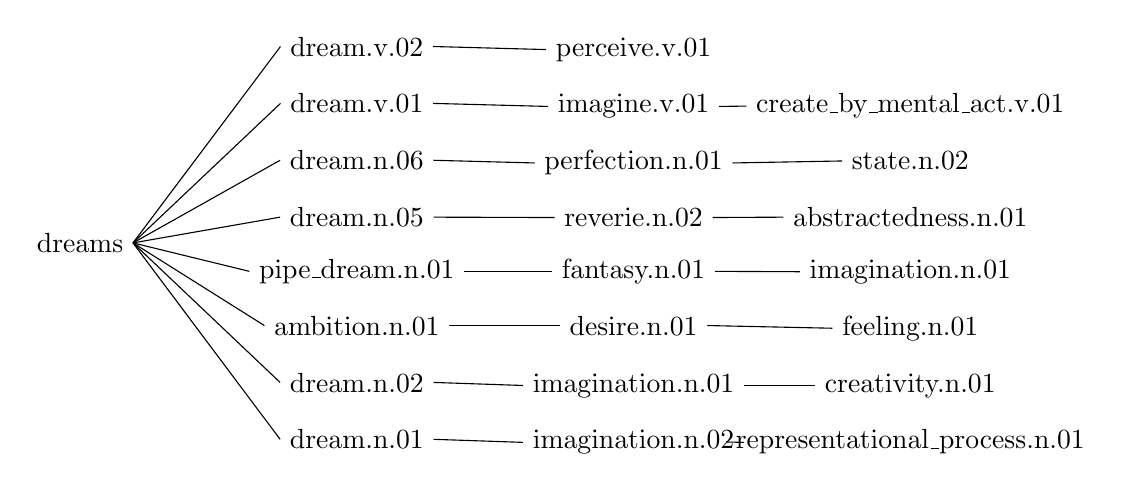
\begin{tikzpicture}[grow=right, sibling distance=5pt, level distance=100pt]
\Tree [.dreams [.dream.n.01 [.imagination.n.02 representational{\_}process.n.01 ] ] [.dream.n.02 [.imagination.n.01 creativity.n.01 ] ] [.ambition.n.01 [.desire.n.01 feeling.n.01 ] ] [.pipe{\_}dream.n.01 [.fantasy.n.01 imagination.n.01 ] ] [.dream.n.05 [.reverie.n.02 abstractedness.n.01 ] ] [.dream.n.06 [.perfection.n.01 state.n.02 ] ] [.dream.v.01 [.imagine.v.01 create{\_}by{\_}mental{\_}act.v.01 ] ] [.dream.v.02 [.perceive.v.01 ] ] ]
\end{tikzpicture}
\caption{HYPERNYM TREE OF "DREAMS"}
\label{fig:hypernymTree}
\end{figure}

\begin{figure}[h]
	\includegraphics[scale=0.6]{HypernymActivation.png}
	\caption{HYPERNYM ACTIVATION}
	\label{fig:HypernymAct}
\end{figure}

Upon activation, the synset in question's activation is increased by an amount, dependant upon the hypernym model used (discussed later in this section). The same synset can be activated multiple times within the same sentence, an example of which is shown in Figure \ref{fig:HypernymAct}. In this case, a similar model to \hyperref[sec:MattBurke]{that proposed by M. Burke} \cite{MattBurkePrevious} is used: 
\[H = \sum\limits_{i=1}^N S_i\] 
The total acivation increase is equal to the sum of all synset activations within the sentence. 

It can be seen that, in Listing \ref{lst:HypernymActivation},there exists a function, hypernymModel. This function is responsible for reducing the activation increase of hypernyms as they become more general (closer to the top of the tree). This function should favour most heavily, less general hypernyms, i.e. those activated by the first few recursions of activateHypernyms. 

\begin{figure}[h]
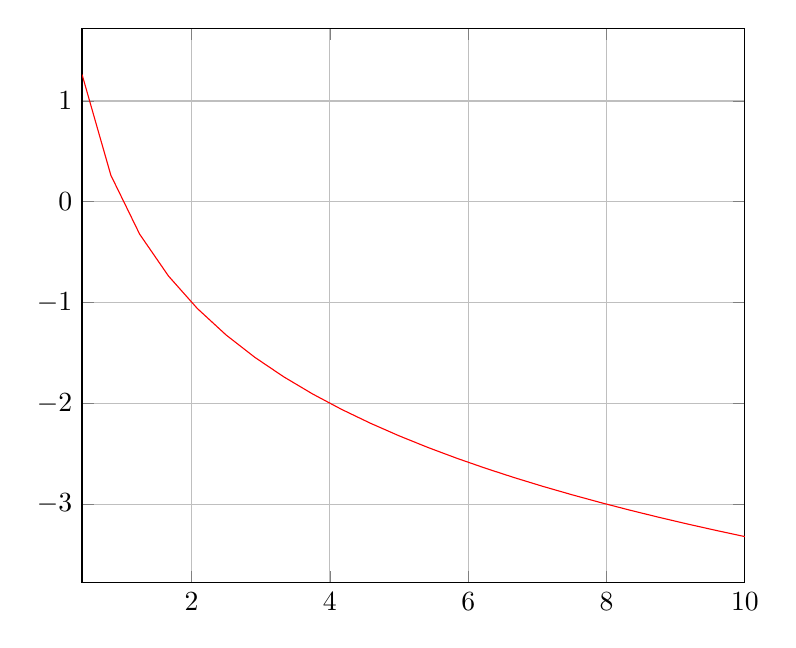
\begin{tikzpicture}
\begin{axis}[domain=0:10, grid=both, enlarge x limits=false]
\addplot[color=red]{-log2(x)};
\end{axis}
\end{tikzpicture}
\caption{GRAPH OF $-\log(x)$}
\label{fig:logGraph}
\end{figure}

One function which fits this criteria is $-\log(x)$, shown in Figure \ref{fig:logGraph}. The values given by the function, for higher values of $x$ are relatively high, favouring more general hypernyms heavily. For lower values of $x$, the values given are relatively low, causing more general hypernyms to have a lower activation increase.

It may be necessary to tune this function during experimentation, to provide greater accuracy, meaning more variables must be added. With these additions, the full model is:
\[f(x) = -b\log(ax)\]
where $a$ and $b$ are varied during experimentation, and $x$ is the depth of the hypernym. When the depth = 0 (i.e. the activation of the root synset) the model would require the calculation of log(0), which is undefined. For this reason, an offset of 0.001 was added, making the final model:
\[f(x) = -b\log(ax+0.001)\]
The size of the offset needed to be small to reduce its impact on the overall model.


\subsection{Memory Structures}
\label{sec:ImplementedMemoryStructures}

Upon activation, the synset in question may enter the memory structures, if it posesses a high enough activation. Both an STS and Episodic Buffer have been implemented, using python classes for each. Interactions between the two memory structures are handled by a Memory Controller. As discussed in the \hyperref[Wordnet]{WordNet section}, WordNet provides a good model of the semantic memory \cite{WN1Introduction},described in the \hyperref[LongTerm]{Long-term Store section}. For this reason it has been used heavily.

\subsubsection{STS}
\label{sec:ImplementedSTS}

The STS (Stm in psuedocode) can, in a simplified sense, be described as a list containing memory items. These memory items have been implemented in python as an object with two attributes, synset (immutable) and activation (mutable), based upon the contents of the STS in the working memory model. These memory items can be replaced, if a synset with greater activation appears. The process of synset replacement is handled by the swapLowestItem function shown in Listing \ref{lst:swapLowestItem}.

\begin{lstlisting}[numbers=left, numberstyle=\small, caption={the swapLowestItem function}, captionpos=b, label={lst:swapLowestItem}]
FUNCTION swapLowestItem(newItem):
        IF Stm.size < self.maxStmSize THEN
            Stm.add(newItem)
            RETURN None
        ELSE
            self.lowestItem = self.getLowestActivation()
            IF newItem.Activation < stm.lowestActivationItem THEN
                RETURN None
            ELSE
                Stm.remove(lowestActivationItem)
                Stm.add(newItem)
                RETURN stm.lowestActivationItem
            END IF
        END IF
END FUNCTION
\end{lstlisting}

A notable feature of the STS is its limited capacity, as described by G. Miller in 1955 \cite{SevenPlusMinusTwo}. It is for this reason that the ability to swap memory items is required. In the case that the STS isn't full, the new memory item is simply added with no swap taking place.

\subsubsection{Episodic Buffer}
\label{sec:ImplementedEpisodicBuffer}

The purpose of the episodic buffer, is to maintain a list of synsets which have occurred in the STS previously. This allows future activations of synsets which have already occured to receive a boost when activated in the future. Interactions with the Episodic buffer only occcur during the activation of synsets, therefore, all interactions are handled by the Memory Controller.

\subsubsection{Semantic Memory}
\label{sec:ImplementedSemanticMemory}

The Semantic Memory is responsible for maintaining all the semantic knowledge of the system. It was decided that WordNet provided the best solution, with its in depth knowledge of synsets and their relations to eachother \cite{WN2Nouns, WN4Verbs}.

NLTK's built in WordNet reader \cite{NLTK} was used to interact with WordNet. Throughout the system, synsets are used. Each of these is a reference to a synset present in WordNet, allowing their semantic relationships (accessed through their methods) to be used. 

\subsubsection{Memory Controller}
\label{sec:ImplementedMemoryController}

A memory controller has been implemented to handle interactions between the STS and episodic buffer. The most notable of its uses is the activation of synsets. In order to activate a synset, the Memory Controller must take into account the whether the synset is present in any of the afformentioned memory structures, and handle the activation accordingly. The activateSynset function, shown in Listing \ref{lst:activateSynset} is responsible for handling this process.

\begin{lstlisting}[numbers=left, numberstyle=\small, caption={the activateSynset function}, captionpos=b, label={lst:activateSynset}]
FUNCTION activateSynset(self, synset, activationModifier):
        IF stm.inContents(synset) THEN
            synset.activate(activationModifier)
            RETURN
        ELSE IF episodicBuffer.inContents(synset) THEN
            newMemItem = MemItem(synset, 1)
            newMemItem.activate(activationModifier)
            sendToStm(newMemItem)
            RETURN
        ELSE
            newMemItem = MemItem(synset, 0)
            newMemItem.activate(activationModifier)
            sendToStm(newMemItem)
            RETURN
        END IF
\end{lstlisting}

If the activateSynset finds the synset in the STS, the synset is simply activated using, and remains there. If the synset is not present in the STS, it is activated, and sent to the STS, through the sendToStm function, shown in Listing \ref{lst:sendToStm}, recieving a boost if it has previously existed in the STS (i.e. it is in the Episodic Buffer).

\begin{lstlisting}[numbers=left, numberstyle=\small, caption={the sendToStm function}, captionpos=b, label={lst:sendToStm}]
FUNCTION sendToStm(inputSynset):
	returnedItem = self.stm.swapLowestItem(inputItem)
    IF returnedItem is None THEN
        RETURN
    ELSE IF NOT episodicBuffer.inContents(returnedItem) THEN
        episodicBuffer.addSynset(returnedItem)
        RETURN
    END IF
END FUNCTION
\end{lstlisting}

The sendToStm function, shown in Listing \ref{lst:sendToStm}, is responsible for changing the contents of the STS and updating the Episodic buffer accordingly. The swapLowestItem function, shown in Listing \ref{lst:swapLowestItem} is used to edit the STS. As discussed \hyperref[sec:ImplementedSTS]{previously}, this function can return a synset, if the swap is successful. In this case, sendToStm will add the synset previously in the STS, to the episodic buffer (if it is not already present there).

Throughout the analysis of a corpus, the activation of a specific memory item can change by either being forgotten or activated.

\subsection{Forgetting}
\label{sec:forgetting}
After each sentence is read, all items in the STS must be forgotten (have their activation reduced), so as to comply with Atkinson and Shiffrin's STS model discussed \hyperref[ShortTerm]{previously} \cite{ControlProcessesSTMAtkinson}. The forgetting of the entire contents of the STS is done using a loop, as shown in Listing \ref{lst:ForgetLoop}.

\begin{lstlisting}[numbers=left, numberstyle=\small, caption={Forget loop}, captionpos=b, label={lst:ForgetLoop}]
FOR item IN Stm LOOP
	item.forget()
END LOOP
\end{lstlisting}

The forgetting process occurs after every sentence, giving synsets in the next sentence the opportunity to enter the STS.

When a synset is forgotten, its activation may fall below a threshold, varied in experimentation. If this occurs, the synset is removed from the STS and, as with the sendToStm function, is added to the Episodic Buffer. This prevents synsets irrelevant to the current context from existing in the STS.

\subsection{Disambiguation}
\label{sec:ImplementedDisambiguation}
Up to this point, we have only discussed the processes involved with changing the contents of the memory structures. The purpose of these memory structures is to provide the surrounding context of a word, to aid in its disambiguation. There exists a delay between the processes described previously (i.e. the initial reading of the sentence) and the disambiguation phase. This delay allows inappropriate synsets to leave the STS before they are used. The duration of this delay is to be adjusted during experimentation.

As discussed in the \hyperref[sec:DisambiguationModels]{Disambiguation Models section}, the multiple access model relies upon context and frequency, using whichever is stronger for disambiguation \cite{PsychologyOfLanguage}. The system discussed in this section makes use of both of these, through the disambiguate function, shown in Listing \ref{lst:disambiguate}.

\begin{lstlisting}[numbers=left, numberstyle=\small, caption={The disambiguate function}, captionpos=b, label={lst:disambiguate}]
FUNCTION disambiguate(synsetList):
    FOR item in stm LOOP
        IF item in synsetList THEN
            RETURN item
        END IF
    END LOOP
    FOR item in stm LOOP
        returnedSynset = hyponymSearch(synsetList, item)
        IF returnedSynset is not None THEN
            RETURN returnedSynset
        END IF
    END LOOP
    RETURN mostLikelySynset(synsetList)
END FUNCTION
\end{lstlisting}

\subsubsection{Context}
\label{sec:DisambiguationContext}
The context used for disambiguation its taken from two sources, the STS and knowledge of noun-verb relationships (the latter is discussed in the \hyperref[Sanity]{Sanity Checking Section}).

Initially, the context contained in the STS is used. Two algorithms for disambiguation using this context have been implemented, one using hyponyms and one using hypernyms.

As discussed in the \hyperref[sec:MattBurke]{Previous Works section}, M. Burke found that hyponym based searching (previously called STM-First), using the Stm is the most effective method of disambiguation \cite{MattBurkePrevious}. This method works upon the assumption that the contents of the Stm are relatively general (i.e. exist high up in the Wordnet hierarchy). The implementation of this search is given by the hyponymSearch function, shown in Listing \ref{lst:hyponymSearch}.

\begin{lstlisting}[numbers=left, numberstyle=\small, caption={The hyponymSearch function}, captionpos=b, label={lst:hyponymSearch}]
FUNCTION hyponymSearch(synsetList, searchItem):
    hyponymList = searchItem.hyponyms()
    IF len(hyponymList) == 0 THEN
        RETURN None
    END IF
    FOR item in hyponymList LOOP
        IF item in synsetList THEN
            RETURN item
        END IF
    END LOOP
    FOR item in hyponymList LOOP
        returnedItem = hyponymSearch(synsetList, item)
        IF returnedItem is not None THEN
            RETURN returnedItem
        END IF
    END LOOP
    RETURN None
\end{lstlisting}

This function traverses through all hyponyms of a given synset (searchItem) until either, a match with a synset in the synsetList is found, or the function reaches the base of the tree. If a match is found, the matched synset is returned as the correct word meaning.

Another algorithm, shown in Listing \ref{lst:hypernymSearch}, for disambiguation has also been implemented, using the lowest{\_}common{\_}hypernym method implemented in NLTK's WordNet reader \cite{NLTK}. This algorithm instead searches the hypernyms of both the word to disambiguate and the item in the STS, to find whether a common hypernym exists. If a common hypernym does exist, it is checked to ensure it is not too general (e.g. the common hypernym could be "entity" which is a hypernym of all nouns), and the synset is returned as the correct meaning.

\begin{lstlisting}[numbers=left, numberstyle=\small, caption={THE HYPERNYMSEARCH FUNCTION}, captionpos=b, label={lst:hypernymSearch}]
FUNCTION hypernymSearch(synsetList, searchItem):
    FOR synset in synsetList LOOP
        common_hypernym = synset.lowest_common_hypernym(searchItem)
        IF common_hypernym.depth > 4 THEN
            RETURN synset
       	END IF
   	END LOOP
\end{lstlisting}  

Using either method, a meaning will only be found if the surrounding context of a word gives enough indication of its meaning, complying with the multiple access model, where if strong context exists, it is used for disambiguation \cite{PsychologyOfLanguage}.

\subsubsection{Frequency}
\label{sec:DisambiguationFrequency}
The previously described hyponym-based system will only find a meaning if a word's surrounding context is strong. When this is not the case, another system must be used. The multiple access model, described in the \hyperref[sec:DisambiguationModels]{Disambiguation Models section}, states that in such cases, the likelihood of a proposed word meaning is used \cite{PsychologyOfLanguage}.

In order to calculate the likelihood of each synset in the synsetList, Wordnet's lemmas are used. Lemmas in Wordnet are the word forms a synset can take. For each lemma, there exists a frequency value, which describes how common that form is, relative to other Wordnet lemmas. For each synset, the sum of all its lemmas' frequency values, is used to calculate the most likely synset, as shown in Listing \ref{lst:synsetFrequency}.

\begin{lstlisting}[numbers=left, numberstyle=\small, caption={The synsetFrequency and mostLikelySynset functions}, captionpos=b, label={lst:synsetFrequency}]
FUNCTION synsetFrequency(synset):
    outputFrequency = 0
    FOR lemma in synset.lemmas() LOOP
        outputFrequency += lemma.count()
    END LOOP
    RETURN outputFrequency
END FUNCTION

FUNCTION mostLikelySynset(synsetList):
    outputSynset = synsetList[0]
    FOR synset in synsetList LOOP
        IF synsetFrequency(outputSynset) < synsetFrequency(synset) THEN
            outputSynset = synset
        END IF
    END LOOP
    RETURN outputSynset
END FUNCTION
\end{lstlisting}

As stated previously, in cases where context cannot provide a viable synset, the above is used for disambiguation.

\subsubsection{Sanity Checking}
\label{Sanity}
Given the sentence:
\[He\: fixed\: the\: bug\]
The reader knows that "bug" refers to a computer bug, due to its use with the verb "fixed". So far, the system has no way of modelling the contextual effects of nouns on verbs, so the system is likely to produce invalid sentences. For this reason, post-disambiguation sanity checks occur.

Though a proposed feature, WordNet does not currently contain relationships between nouns and verbs \cite{WN4Verbs}. For this reason, the information had to be extracted from the available corpus. It was decided that half of the test corpus would be used for the extraction, so that test data used for evaluation would be completely new to the system.

Listing \ref{lst:verbDistance} shows the algorithm used for extracting this information. Nouns which occur in the same sentence as a specific Verb are considered valid partners to the Verb, and are added to a dictionary for quick lookup.

\begin{lstlisting}[numbers=left, numberstyle=\small, caption={The noun-verb relationship learning algorithm}, captionpos=b, label={lst:verbDistance}]
FUNCTION verbDistance(verb, sentence):
	FOR word in sentence LOOP
		IF word is a noun THEN
			outputList.append(word.synset)
		END IF
	END LOOP
	RETURN outputList
END FUNCTION			

FOR sentence in inputCorpus LOOP
	FOR every verb in sentence LOOP
		update contents of verbDict[verb.synset] 
		to include verbDistance(verb, sentence)
	END LOOP
END LOOP
\end{lstlisting}

Initially, the sentence is disambiguated, using the method described \hyperref[sec:ImplementedDisambiguation]{previously}. The outputted sentence is then checked for correctness by the function sanityCheck, as shown in Listing \ref{lst:sanityCheck}. If a synset is found to be incompatible with others in the sentence, it is added to a blacklist, and its corresponding word is disambiguated again, ignoring the previous meaning.

\begin{lstlisting}[numbers=left, numberstyle=\small, caption={The sanityCheck function}, captionpos=b, label={lst:sanityCheck}]
FUNCTION sanityCheck(inputSentence, nounDict, verbDict):
    sane = False
    FOR word in inputSentence LOOP
        IF word is a noun THEN
            nounList.append(word)
        ELSE IF word is a verb THEN
            verbList.append(word)
        END IF
    END LOOP
    WHILE not sane LOOP
        sane = True
        FOR verb in verbList LOOP
            IF verb in verbDict THEN
                plausibleNouns =  verbDict[verb]
                IF nounList and plausibleNouns share common words THEN
                    verbList.remove(verb)
                ELSE
                    blackList.append(verb)
                    verbList.remove(verb)
                    Run disambiguation again with blacklist
                END IF
            END  IF
		END LOOP
	END LOOP
END FUNCTION
\end{lstlisting}

It may be noted that sanityCheck only considers verb incorrectness. As stated in the \hyperref[Verbs]{WordNet section}, for each word, there is likely to be a larger set of synsets when compared to nouns. With this knowledge, we can assume that the likelyhood of an incorrect result for a verb is higher than that of a noun. 



\section{Results and Evaluation}
\label{sec:Results}

\section{Conclusions}
\label{sec:Conclusions}

\newpage
\bibliography{references}
\bibliographystyle{IEEEtran}

\end{document}